\documentclass{jreport}
\usepackage[dvipdfmx]{graphicx}
\usepackage{cases}


\begin{document}
\title{理学総論レポート(担当:河野先生)}

\author{お茶の水女子大学人間文化創成科学研究科理学専攻 \\1940620 \\ 前田実津季}
\date{\today}
\maketitle

\subsection*{1.散乱実験に関して}
\noindent
ATLAS実験に関して論じる。\\
ATLAS実験は、CERNのLHCで行われている世界最大の加速器実験である。\\
LHCは、全周が山手線1周ほどの約27kmの加速器である。スイスとフランスの国境の地下100m付近に加速器であるトンネルが位置している。ここで、陽子同士を加速させ、正面衝突させている。LHCには、図のように、4つの巨大な検出器があり、ATLAS、CMS、ALICE、LHCbと分かれている。\\
\begin{figure}[htbp]
	\begin{center}
	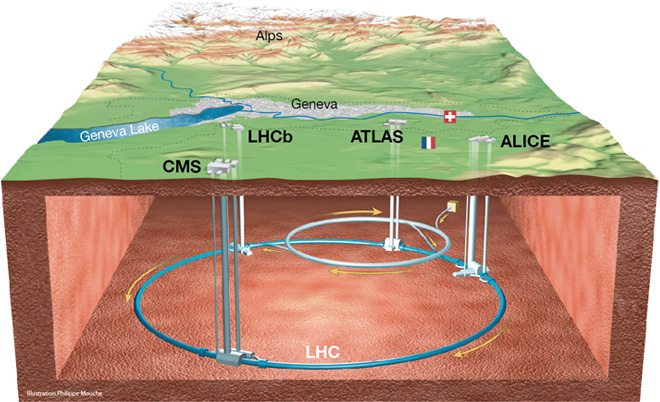
\includegraphics[width=100mm]{image_atlas_02.jpg}
	\end{center}
	\caption{LHCのイメージ図}
	\label{fig:one}
\end{figure}
このLHCの衝突エネルギーは、2015年〜2018年のRun2の期間では、設計値に近い13TeVまで上げて実験を行なっていた。2019年〜2020年の運転停止期間には2021年〜2023年のRun3に向けての増強開発が進められている。このRun3では、衝突エネルギーは14TeVで実験が再開される。\\

このLHCの検出器の1つにATLAS検出器がある。この検出器は、高さ25m、長さ44m、重さ7000tの巨大な検出器である。検出器の構成としては、内側から、内部飛跡検出器、電磁カロリーメータ、ハドロンカロリーメータ、ミューオン検出器という構造になっている。これらの検出器で、粒子の運動量やエネルギーを測定し、各事象の生成・崩壊過程を観測する。
\begin{figure}[htbp]
	\begin{center}
		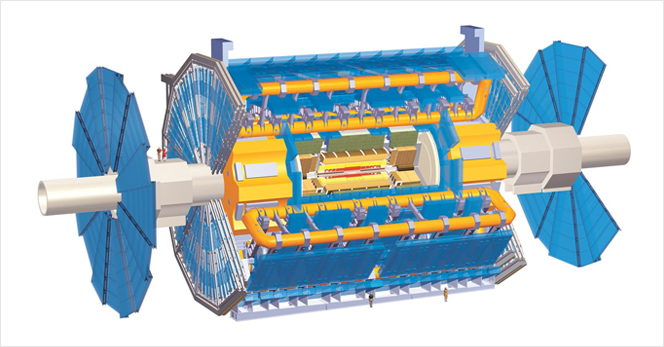
\includegraphics[width=100mm]{image_atlas_03.jpg}
	\end{center}
	\caption{ATLAS検出器の構成図}
	\label{fig:two}
\end{figure}

\newpage
\subsection*{2.対象しているものに関して}
\noindent
ATLAS実験では、陽子同士の衝突実験から観測される事象から検出される物理量を用いて、2012年には、ATLAS実験とCMS実験にて新粒子であるヒッグス粒子の発見に貢献しました。\\
現在標準理論の精密測定や、標準理論を超える新物理の探索を行うため実験を行なっている。特にLHCでは、世界最大のエネルギースケールを誇り、これまでのエネルギースケールでは、よくわからなかった重いトップクォークや、ヒッグス粒子などの精密測定に力を注いでいる。\\
これまでに実験よって存在を確認できた素粒子を図に示す。
\begin{figure}[htbp]
	\begin{center}
		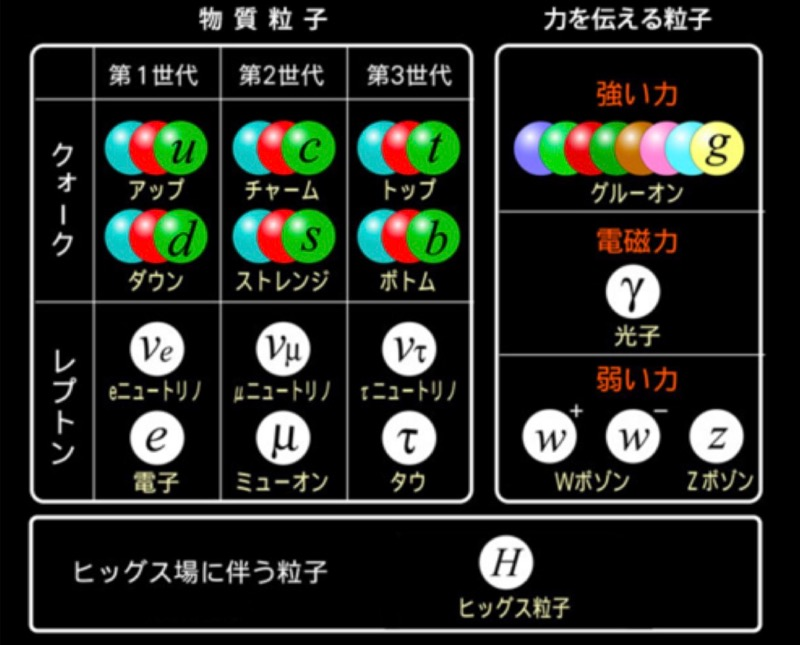
\includegraphics[width=70mm]{001l.jpg}
	\end{center}
	\caption{これまでに確認された素粒子}
	\label{fig:three}
\end{figure}
\subsection*{3.対象を調べる取り組みに関して}
\noindent
実験における粒子の物理量の検出の仕組みに関して述べる。特に、事象の理解には、生成された粒子の飛跡、運動量、エネルギーの検出が重要になってくる。そのため、それぞれの検出器によって物理量を検出する仕組みについて見ていく。\\
内側から、まず内部飛跡検出器は、荷電粒子の運動量と飛跡の測定を行なっている。内部飛跡検出器は、ピクセル検出器、シリコン検出器、遷移輻射検出器の3つの検出器で構成されている。一般的な運動量と位置の測定方法を述べる。\\
\begin{figure}[htbp]
	\begin{center}
	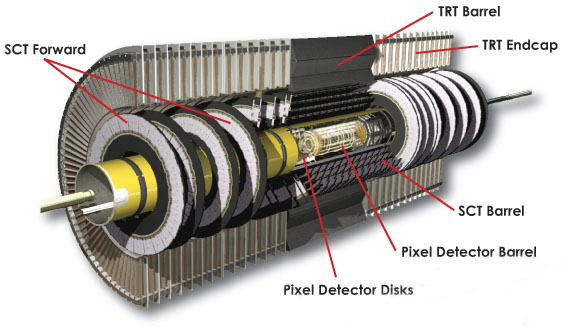
\includegraphics[width=70mm]{image4.jpg}
	\end{center}
	\caption{内部飛跡検出器}
	\label{fig:four}
\end{figure}
\\
内部飛跡検出器の外側には、ソレノイド磁石が設置されており、磁場(2T)をかけている。この磁場によって荷電粒子は曲げられ、その飛跡を測定することで、運動量の測定を行なっている。\\
荷電粒子の磁場中の運動方程式は、次のようにかける。\\
\begin{eqnarray}
\frac{mv^2}{R} &=& evB \\
R &=& \frac{p}{eB}
\end{eqnarray}
ATLAS実験のような高エネルギーの実験では、次のように運動方程式を書き直すことができる。
\begin{eqnarray}
R[m] &=& \frac{p[GeV/c]}{0.3 B[T]} \\
p &=& 0.3 B R
\end{eqnarray}
つまり、運動量は、磁場の強さと飛跡の半径(R)が分かれば求まる。\\
実際の測定には、サジッタと呼ばれる量を使用して、運動量の測定を行なっている。図5のLは、粒子を各検出器で測定した点を飛跡としてつなげた始点と終点までの直線距離である。またRは、ビーム軸の中心からヒットした点までの距離であり、飛跡の曲線の半径である。\\
図5の右図内の直角三角形から、R、s、Lとの関係について示すと、
\begin{eqnarray}
	R^2 &=& (R-s)^2 + (\frac{L}{2})^2 \nonumber \\
	R &=& \frac{L^2}{2s}+\frac{s}{2} \nonumber \\
	s \ll L より && \nonumber \\
	R &\simeq& \frac{L^2}{2s}
\end{eqnarray}
となり、つまり測定した運動量は、次のように求まる。
\begin{eqnarray}
	p = 0.3 B \frac{L^2}{2s}
\end{eqnarray}
よって、粒子がヒットした位置を使用して、Lとsの量がわかると、運動量が求まる。

\begin{figure}[htbp]
	\begin{center}
	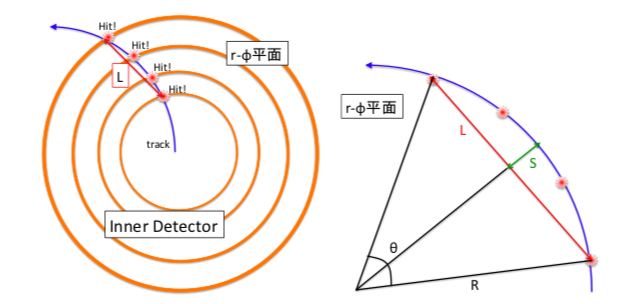
\includegraphics[width=100mm]{sagitta.png}
	\end{center}
	\caption{飛跡の測定}
	\label{fig:five}
\end{figure}
次に、カロリーメータがある。カロリーメータは、電磁カロリーメータとハドロンカロリーメータの2つに分類することができる。それぞれのカロリーメータの役割と検出方法についてまとめる。\\
\begin{figure}[htbp]
	\begin{center}
	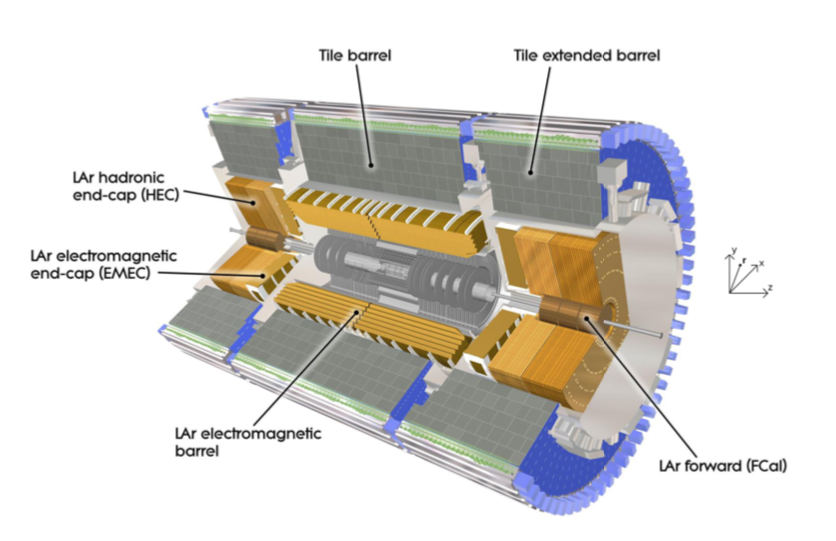
\includegraphics[width=90mm]{calorimeter.png}
	\end{center}
	\caption{カロリーメータ}
	\label{fig:five}
\end{figure}
\\
\newpage
電磁カロリーメータでは、電子、光子を、ハドロンカロリーメータではハドロンのエネルギーを測定している。粒子のエネルギーを測定するために、粒子をカロリーメータ内で止める必要がある。よって、カロリメータは、鉛や鉄などの物質量の大きな材質で構成されている。\\
電磁カロリーメータでは、電子と光子は、カロリーメータを構成する物質との電磁相互作用によってエネルギーを落としていく。また、電子と光子はそれぞれカロリーメータ内でエネルギーを落としていく過程での飛跡の違いから同定することができる。\\
ハドロンカロリーメータでは、ハドロンが強い相互作用や、電磁相互作用、原子核の衝突によってエネルギーを落とし、ハドロンカロリーメータ内で止まる。
\\
\\
最後に、ミューオンスペクトロメータである。ここでは、ミューオンの測定を目的としており、位置の精密測定や運動量の測定を行なっている。
ミューオンは、検出器の外部に設置されているトロイドコイルによる磁場によって曲げられ、内部飛跡検出器の荷電粒子の運動量検出と同様に運動量が再構成される。

\subsection*{4.測定装置の改善によって新たな地平を切り開く可能性に関して}
\noindent
測定装置の改善に関して、現状の測定器に関する懸念点と、それに対する解決案、将来の展望を述べる。\\
現に、ATLAS実験では、実験の開始から徐々に衝突させる陽子の衝突エネルギーとルミノシティ を上げて、実験を行なっている。それは、より高いエネルギースケールでしか分からない重い粒子の精密測定であったり、今までのエネルギースケールでは見えてこなかった新物理の探索であったりを行うためである。加えて、より注目するイベント数を増やして解析を行うためである。\\
そして、衝突エネルギーとルミノシティ をあげるに当たって、必要となるのが測定器のアップグレードである。このルミノシティ と衝突エネルギーをあげたLHCをHL-LHCと呼ぶが、HL-LHCでは、衝突により引き起こされるイベント数も膨大になり、それに比例して、検出器に入射する粒子も増える。検出器に使用されているセンサーの小型化に伴う読み出しチェンネルの増加はもちろんであるが、入射粒子の増加に伴い、検出器の放射線環境が過酷となる。そのため、特に内部に位置する検出器の内部飛跡検出器のアップグレードが現在行われている。\\
そのため、今回は、内部飛跡検出器の放射線損傷に関して述べ、アップグレードに沿ってどのように検出器をリニューアルする必要があるのかを考える。\\
まず、内部飛跡検出器は、シリコンを用いた半導体検出器である。半導体検出器は、正孔が電荷の担い手になっているp型半導体と、価電子が1つ多く、この電子が電荷の担い手になっているn型半導体を接合させることで、空乏層を作る。また、このpn接合をした半導体に逆バイアスをかけることで空乏層を広げ、全空乏化して、センサーとして用いている。\\
\begin{figure}[htbp]
	\begin{center}
	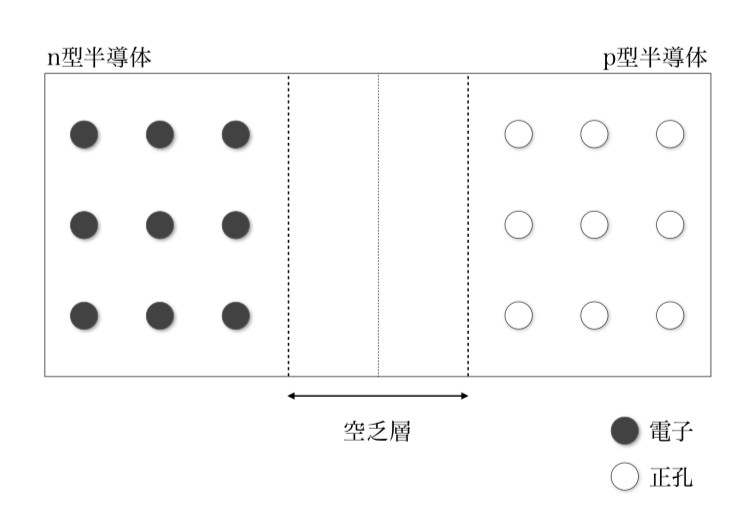
\includegraphics[width=100mm]{silicon.png}
	\end{center}
	\caption{pn接合に空乏層の様子}
	\label{fig:six}
\end{figure}
この空乏層に荷電粒子が通過する時に、電子・正孔対を生成し、これらの電荷を収集することで粒子通過の信号として読み出して粒子の位置を測定している。\\
このシリコン検出器の放射線損傷としては、2つに分類することができる。表面損傷とバルク損傷である。今回は、バルク損傷に注目して、検出器への影響をまとめる。バルク損傷とは、シリコンセンサーのバルク部分の原子と入射粒子との相互作用により格子欠陥が生成されることである。\\
\begin{figure}[htbp]
	\begin{center}
	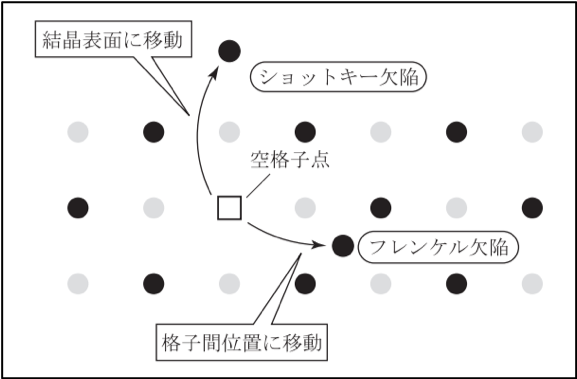
\includegraphics[width=100mm]{kekkan.png}
	\end{center}
	\caption{放射線損傷による引き起こる欠陥}
	\label{fig:seven}
\end{figure}
\\
図が、実際入射粒子による格子欠陥の様子である。\\
\\
*暗電流の増加 - 禁止帯に新たなエネルギー準位ができることにより、価電子帯から伝導帯への遷移確率が増大する。暗電流の増加は、放射線量に比例する。\\ 
*バルクの型変換 - センサーが放射線を受け、n型のバルク部にp型不純物として振る舞う格子欠陥が生成される。不純物が増えるとやがてバルクはp型になり、型変換が起こる。 \\ 
*全空乏化電圧の増加 - 有効不純物密度に比例するため。$v_{fd} \sim \frac{ed^2}{2\epsilon_{si}}|N_{eff}| $ \\ 
*電荷収拾量の減少 - 新たなエネルギー準位により、荷電粒子によって生成される電子ホール対は、そのエネルギー準位に捕獲、再結合される確率が高くなる。つまり信号量が低下する。\\

このような格子欠陥が増える中で、行う処理としては、アニーリングがある。アニーリングとは、原子の熱振動により放射線損傷による格子欠陥が移動し、その際に格子欠陥が消滅することで有効不純物濃度が減少する現象である。半導体の温度を上げ続けると、逆アニーリングと呼ばれる逆に有効不純物濃度が増加する現象が見られるので、温度を上げれば良いというものではない。\\
次の図は、60℃でアニーリングを行なった際の時間における有効不純物濃度の変化を表している。\\
\begin{figure}[htbp]
	\begin{center}
	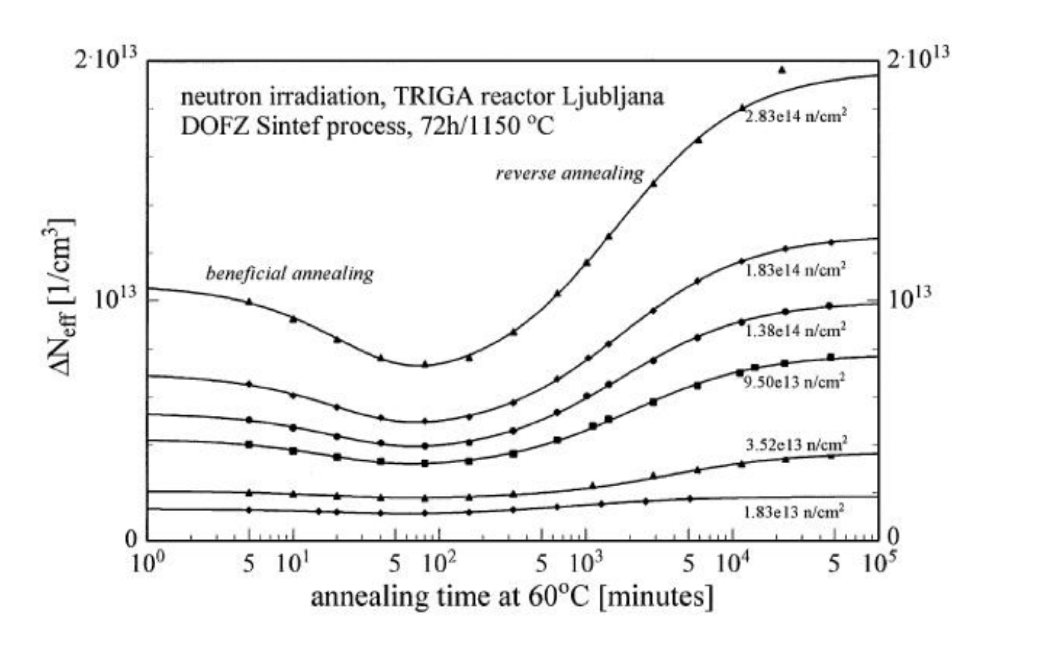
\includegraphics[width=100mm]{annealing.png}
	\end{center}
	\caption{アニーリング処理と時間の関係}
	\label{fig:eight}
\end{figure}
\\
一般的にアニーリングには60~80℃で行われる。この処理によって放射線損傷による格子欠陥が減少が見込まれるが、今後のATLAS実験のアップグレードにおける検出器の改善としては、高い放射線耐性である。\\
高い放射線耐性のセンサーの開発としての取り組みの1つとしては、例えば、センサーの構造の改善などがある。\\
現在実験に使用しているセンサーとしては、p-in-nのセンサーである。この場合は、図のように読み出し電極側にpn接合面があり、電極側に空乏層が広がる。放射線損傷が起こると、読み出し電極の反対側から空乏層が広がるようになる。このため、型変換が起こると、信号を読み出すためには、センサーの全空乏化が必要になる。\\

\begin{figure}[htbp]
	\begin{center}
	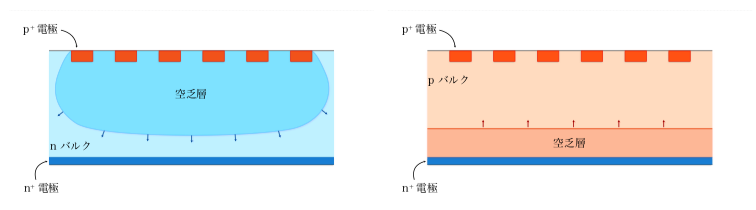
\includegraphics[width=100mm]{pn.png}
	\end{center}
	\caption{p-in-nセンサーの空乏層が広がる様子}
	\label{fig:nine}
\end{figure}

しかし、n-in-pセンサーの場合は、まずバルク部がp型のため型変換が起きない。読み出し電極側から空乏層が広がるため、全空乏化しなくても信号を読み出すことができる。加えて、読み出し電極がn型の半導体である。そのため、信号として収集する電荷は正孔ではなく、電子である。結晶中での移動度は、正孔よりも電子の方が大きいため放射線損傷による格子欠陥などにトラップされにくいと考えることができる。\\
\begin{figure}[htbp]
	\begin{center}
	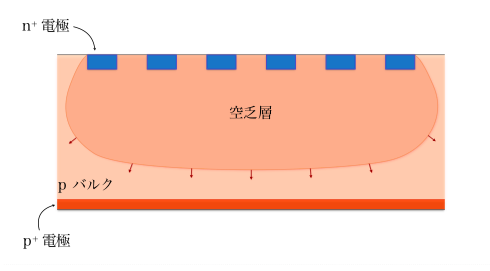
\includegraphics[width=100mm]{n-in-p.png}
	\end{center}
	\caption{n-in-pセンサーの様子}
	\label{fig:ten}
\end{figure}
\\
上記の理由からn-in-pセンサーよりもp-in-nセンサーの方が放射線耐性が高い。\\
これは1つの放射線耐性を高める開発であるが、このようにより放射線耐性の高い検出器が求められている。検出器を構成する物資で、より放射線耐性の高い物質でのモジュールの製作への研究なども行われている。\\
他にもアップグレードに向けて、より早く信号の読み出しに向けた研究や、センサーの小型化なども必要な改善である。



\end{document}